\documentclass[11pt]{article}
\textwidth 17cm
\textheight 23cm
\oddsidemargin 0.25cm
\addtolength{\voffset}{-2.4cm}
\addtolength{\hoffset}{-0.5cm}
\setlength{\parindent}{12pt}
\setlength{\parskip}{3pt}
\usepackage{amssymb,amsmath,epsfig,graphics,psfrag,graphicx,color,cite,subfigure,amsthm}
\usepackage[colorlinks=false,breaklinks=true,linkcolor=blue]{hyperref}
\numberwithin{equation}{section}
\usepackage{cleveref}
%\usepackage{refcheck}

% OUR DEFINITIONS %%%%%%%%%%%%%%%%%%%%%%%%%%%%%%%%%%%

\usepackage{mathtools}
\makeatletter
\newcommand{\vast}{\bBigg@{4}}
\newcommand{\Vast}{\bBigg@{5}}
\makeatother


\newtheorem{thm}{Theorem}[section]
\newtheorem{rem}{Remark}[section]
\newtheorem{lem}[thm]{Lemma}
\newtheorem{defi}{Definition}[section]
\newtheorem{prop}{Proposition}[section]


\newcommand{\tr}{\operatorname*{tr}}
\newcommand{\bdiv}{\operatorname*{\mathbf{div}}}
\newcommand{\vdiv}{\operatorname*{div}}


\def\bw{{\boldsymbol{w}}}
\def\b{\boldsymbol}
\def\bnu{{\boldsymbol{\nu}}}
\newcommand\bx{\boldsymbol{x}}
\newcommand\bI{\mathbf{I}}
\newcommand\bL{\mathbf{L}}
\newcommand\bH{\mathbf{H}}
\newcommand\bW{\mathbf{W}^{\mathrm{E}}}
\newcommand\bWP{\mathbf{W}^{\ma}}
\newcommand\beps{\boldsymbol{\varepsilon}}
\newcommand\btheta{\boldsymbol{\theta}}
\newcommand\ff{\boldsymbol{f}}
\renewcommand\gg{\boldsymbol{g}}
\newcommand\nn{\boldsymbol{n}}
\newcommand\bt{\boldsymbol{t}}
\newcommand\cero{\boldsymbol{0}}
\newcommand\OmP{\Omega^{\mathrm{P}}}
\newcommand\OmE{\Omega^{\mathrm{E}}}
\newcommand{\GN}{\Gamma_{\mathrm{N}}}
\newcommand{\GD}{\Gamma_{\mathrm{D}}}
\def\bta{\boldsymbol{\tau}}

\newcommand{\RR}{\mathbb{R}}

\newcommand\cA{\mathcal{A}}
\newcommand\cB{\mathcal{B}}
\newcommand\cC{\mathcal{C}}

\newcommand\be{\boldsymbol{e}}
\newcommand\br{\boldsymbol{r}}

\newcommand\cF{\mathcal{F}}
\newcommand\cG{\mathcal{G}}
\newcommand\cH{\mathcal{H}}
\newcommand\bbP{\mathbb{P}}
\newcommand\cP{\mathcal{P}}
\newcommand\cT{\mathcal{T}}

%Paired delimiters
\DeclarePairedDelimiter\norm{\lVert}{\rVert}
\DeclarePairedDelimiter\abs{\lvert}{\rvert}

\numberwithin{equation}{section}
\allowdisplaybreaks



%*****************************************
\title{New fully-mixed finite element approximation of a elasticity-poroelasticity interface problem\thanks{This work was
		partially supported by }}

\author{{\sc Bryan G\'omez-Vargas}\thanks{Secci\'on de Matem\'atica, Sede de Occidente, Universidad de Costa Rica, San Ram\'on, Costa Rica, email: {\tt bryan.gomezvargas@ucr.ac.cr}.}
	\quad
	{\sc Paul E. M\'endez}\thanks{Research Centre on Mathematical Modelling (MODEMAT), Escuela
		Polit\'ecnica Nacional, Quito, Ecuador, email: {\tt paul.mendez01@epn.edu.ec}.}}

\date{\today}
\begin{document}
	\maketitle
	
	\begin{abstract}
		
	\end{abstract}
	\noindent
	{\bf Key words}: Elasticity - poroelasticity coupling; interface problems; mixed formulation; mixed finite element method; error estimation. 
	
	\smallskip\noindent
	{\bf Mathematics subject classifications (2000)}: 65N30, 74A50, 76S05, 74F10.
	
	\maketitle
	
	
	%*****************************************
	\section{Introduction}
	%*****************************************
	%***********************************************************************************
	\subsection{Preliminaries}
	%***********************************************************************************
	Let us denote by $\Omega\subseteq \RR^n$, $n=2,3$, an arbitrary bounded domain with
	polyhedral boundary $\Gamma= \partial \Omega$,  and
	by $\bnu$ the outward unit normal vector on $\Gamma$.  We
	recall the standard notation for Lebesgue spaces $\mathrm L^p(\Omega)$
	and Sobolev spaces $\mathrm H^s(\Omega)$ endowed with the norm
	$\Vert\cdot\Vert_{s,\Omega}$ and seminorm $|\cdot|_{s,\Omega}$.  In
	particular, ${\mathrm H}^{1/2}(\Gamma)$ stands for the space of traces
	of functions of $\mathrm H^1(\Omega)$ and ${\mathrm H}^{-1/2}(\Gamma)$
	denotes its dual. By $\mathbf{M}$ and $\mathbb{M}$ we
	will denote the corresponding vectorial and tensorial counterparts of
	the generic scalar functional space $\mathrm M,$ and by $\| \cdot\|,$ with no subscripts, will stand 
	for the natural norm of either an element or an operator in any  product functional space. 
	In turn, for any vector field $\b v=(v_i)_{i=1,n}$ we set the gradient, divergence and tensor product operators as
	\[
	\nabla \b v \,:=\, \left(\frac{\partial v_i}{\partial x_j}\right)_{i,j=1,n} \quad
	\vdiv\,\b v \,:=\, \sum_{j=1}^n \frac{\partial v_j}{\partial x_j}\quad\mathrm{and}\quad \b v\otimes\bw:=(v_iw_j)_{i,j=1,n}.
	\]
	In addition, for any tensor fields $\bta=(\tau_{ij})_{i,j=1,n}$
	and $\boldsymbol{\zeta} = (\zeta_{ij})_{i,j=1,n}$, we let $\bdiv\,\bta$ be the divergence operator
	$\vdiv$ acting along the rows of $\bta$, and define the transpose, the trace,
	the tensor inner product, and the deviatoric tensor, respectively, as
	\[
	\bta^{\tt t} \,:=\, (\tau_{ji})_{i,j=1,n}, \quad
	\tr(\bta) \,:=\, \sum_{i=1}^n\tau_{ii}, \quad
	\bta:\boldsymbol{\zeta} \,:=\, \sum_{i,j=1}^n\tau_{ij}\zeta_{ij}\,, \quad
	\bta^{\tt d} \,:=\, \bta - \frac{1}{n}\,\tr(\bta)\,\mathbb I\,.
	\]
	Furthermore, we recall that
	\[
	\mathbb{H}(\bdiv;\Omega) \,:=\, \Big\{\bta\in \mathbb L^2(\Omega):  \quad \bdiv\,\bta\in
	\mathbf L^2(\Omega)\Big\}\,,
	\]
	equipped with the usual norm
	\[
	\|\bta\|^2_{\bdiv;\Omega} \,:=\, \|\bta\|^2_{0,\Omega}
	\,+\, \|\bdiv\,\bta\|^2_{0,\Omega}\,,
	\]
	is a standard Hilbert space in the realm of mixed problems. In addition, in what follows $\mathbb I$ stands for the 
	identity tensor in $\RR^{n\times n}$, and $|\cdot|$ denotes both the Euclidean norm in $\RR^n$ and the Frobenius norm in $\RR^{n\times n}$. 
	%*****************************************
	\section{Set of governing equations}\label{sec:model}
	%*****************************************
	\subsection{Model problem and boundary-transmission conditions}
	The elastic-poroelastic interface coupled problem consists of a partition into non-overlapping and connected subdomains
	$\OmE$, $\OmP$ representing zones of non-pay rock (where 
	we will set the equations of linear elasticity) and a reservoir
	(where we aim at solving the poroelasticity 
	equations), respectively. We also assume that the reservoir is
	completely immersed in the overall domain: $\overline{\OmP} \subset  \Omega$, 
	such that the interface between the two subdomains,
	denoted as   $\Sigma=\partial\OmP\cap \partial\OmE$, 
	coincides with the boundary of the  pay zone, as portrayed
	in Figure~\ref{fig:sketch}.  Note that on the interface we consider that 
	the normal unit vector $\nn$ is pointing from $\OmP$ to $\OmE$. 
	
	\begin{figure}
		\begin{center}
			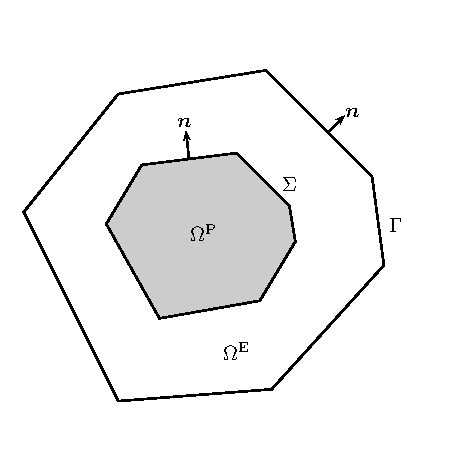
\includegraphics[width=0.575\textwidth]{domain}
		\end{center}
		\caption{Sketch of the multidomain configuration.}\label{fig:sketch}
	\end{figure}
	
	In the reservoir we consider the following balance laws for the
	poroelasticity equations:
	find the poroelastic stress $\b \sigma^{\mathrm{P}}$, the displacement $\b u^{\mathrm{P}}$ and the pore pressure of the fluid $p$ such that
	\begin{align}
	c_0p+\alpha\vdiv(\b u^{\mathrm{P}}) - \frac{1}{\xi}\vdiv \big{[}\kappa(\nabla p
	- \rho \boldsymbol{g})\big{]} &= s & \text{in $\OmP$,}   \label{poro1}\\
	\b \sigma^{\mathrm{P}}  &= 2\mu^{\mathrm{P}}\boldsymbol{\varepsilon}(\boldsymbol{\b u}^{\mathrm{P}})+\lambda^{\mathrm{P}}\vdiv(\b u^{\mathrm{P}})\mathbb{I}-\alpha p\mathbb{I}& \text{in $\OmP$,}  \label{vorm1}\\
	-\vdiv(\b \sigma^{\mathrm{P}}) & = \ff^{\mathrm{P}} & \text{in $\OmP$,} \label{poro3}
	\end{align}
	where $\kappa$ is the
	permeability of the porous matrix constituting the reservoir (here assumed isotropic and
	satisfying $0<\kappa_1\leq \kappa(\bx)\leq \kappa_2<\infty$, for all
	$\bx\in\OmP$), $\lambda,\mu$ are the Lam\'e constants of the solid $\OmP$ (dilation and shear 
	moduli of elasticity, respectively),
	$c_0>0$ is the constrained specific storage coefficient, $\alpha>0$ is
	the Biot-Willis parameter, $\gg$ is the gravity acceleration, 
	and $\xi>0,\rho>0$ are the viscosity and density of the pore fluid, respectively. On the other hand, in $\OmE$ the governing equations correspond to the system of linear elasticity 
	written in terms of stress $\b \sigma^{\mathrm{E}}$, and displacement $\b u^{\mathrm{E}}$,
	associated with the non-pay zone:
	\begin{align}
	\b \sigma^{\mathrm{E}}  &= 2\mu^{\mathrm{E}}\b \varepsilon(\b u^{\mathrm{E}})+\lambda^{\mathrm{E}}\vdiv(\b u^{\mathrm{E}})\mathbb{I}& \text{in $\OmE$,}  \label{elast1}\\
	-\vdiv(\b \sigma^{\mathrm{E}}) & = \ff^{\mathrm{E}} & \text{in $\OmE$,}\label{elast2}
	\end{align}
	where $\mu^{\mathrm{E}}$ and $\lambda^{\mathrm{E}}$ correspond to the Lam\'e constants. Finally, we consider that on the external boundary of the non-pay rock the displacements are zero 
	\begin{equation}\label{eq:bc}
	\b u^{\mathrm{E}}  =\cero \quad \text{on} \quad \Gamma,
	\end{equation}
	and  the system is closed by setting suitable transmission conditions on the interface between the 
	reservoir and the non-pay zone 
	\begin{equation}\label{eq:interface}
	\b u^{\mathrm{P}} = \b u^{\mathrm{E}}, \quad \b \sigma^{\mathrm{P}} \nn = \b \sigma^{\mathrm{E}}\nn , \quad 
	\frac{\kappa}{\xi} (\nabla p - \rho\gg)\cdot\nn = 0, 
	\quad \text{on}\quad \Sigma,
	\end{equation}
	which represent continuity of the medium, matching of total normal stresses, and no-flux of 
	fluid at the interface, respectively.
	
	%*****************************************
	\subsection{Weak formulation}
	%*****************************************
	In this section, we propose a mixed formulation for the coupled interface problem \eqref{poro1}-\eqref{eq:interface}. We start by observing from \eqref{vorm1} and Hooke's law that $$\frac{1}{n\lambda + 2\mu}\mathrm{tr}(\b \sigma^{\mathrm{P}})+\frac{\alpha n}{n\lambda+2\mu}p = \mathrm{div}\,\b u^{\mathrm{P}}, \quad \mathrm{and}\quad \mathcal{C}^{-1}\b \sigma^{\mathrm{P}}=\b \varepsilon(\b u^{\mathrm{P}})-\frac{\alpha}{n\lambda^{\mathrm{P}}+2\mu^{\mathrm{P}}}p\mathbb{I},$$
	from which, the system \eqref{poro1}-\eqref{poro3} can be rewritten  as   
	\begin{align}
	&\Big(c_0+\frac{\alpha^2n}{n\lambda^{\mathrm{P}}+2\mu^{\mathrm{P}}}\Big)p + \frac{\alpha}{n\lambda^{\mathrm{P}}+2\mu^{\mathrm{P}}}\mathrm{tr}(\b \sigma^{\mathrm{P}})- \frac{1}{\xi}\vdiv \big{[}\kappa(\nabla p
	- \rho \boldsymbol{g})\big{]}
	= s&  \text{in $\OmP$,}   \label{poro5}\\
	&\qquad \qquad \qquad \qquad \qquad \qquad \qquad\quad  \mathcal{C}^{-1}\b \sigma^{\mathrm{P}}=\b \varepsilon(\b u^{\mathrm{P}})-\frac{\alpha}{n\lambda^{\mathrm{P}}+2\mu^{\mathrm{P}}}p\mathbb{I}& \text{in $\OmP$,} \label{poro6} \\
	&\qquad \qquad \qquad \quad\;\; \qquad\qquad \qquad\qquad \qquad \qquad \qquad-\vdiv(\b \sigma^{\mathrm{P}})  = \ff^{\mathrm{P}}  & \text{in $\OmP$}. \label{poro7}
	\end{align}
	In this way, recalling that the strain poroelastic tensor can be recast in terms of the gradient and rotation tensors, this is $\b \varepsilon(\b u^{\mathrm{P}})=\nabla\b u^{\mathrm{P}}-\b \omega^{\mathrm{P}},\quad \text{where}\quad \b \omega^{\mathrm{P}}:=\frac{1}{2}(\nabla\b u^{\mathrm{P}}-\nabla ({\b u^{\mathrm{P}}})^{\mathrm{t}}),$ and that $p\mathbb{I}\colon \b \tau = p\tr(\b \tau )\quad \b \tau \in \mathbb{L}^2(\Omega)$, we proceed as usual, testing \eqref{poro5}-\eqref{poro7} by suitable terms, and integrating by parts whenever necessary to obtain 
	\begin{equation}\label{eq:poro-equil}
	\Big(c_0+\frac{\alpha^2n}{n\lambda^{\mathrm{P}}+2\mu^{\mathrm{P}}}\Big)\int_{\OmP}p q+\frac{1}{\xi}\int_{\Omega^{\mathrm{P}}}\kappa\nabla p\cdot \nabla q +\frac{\alpha}{n\lambda^{\mathrm{P}}+2\mu^{\mathrm{P}}} \int_{\OmP} q\,\mathrm{tr}(\b \sigma)=\int_{\OmP}s\,q,
	\end{equation}
	\begin{equation}\label{eq:constitutive-poro}
	\int_{\OmP}\mathcal{C}^{-1}\b \sigma^{\mathrm{P}}\colon\b \tau^{\mathrm{P}} + \int_{\OmP} \b u^{\mathrm{P}} \cdot\mathbf{div}\,\b \tau^{\mathrm{P}} + \int_{\OmP} \b \omega^{\mathrm{P}} \colon\b \tau^{\mathrm{P}} + \frac{\alpha}{n\lambda^{\mathrm{P}}+2\mu^{\mathrm{P}}} \int_{\OmP} p\,\mathrm{tr}(\b \tau^{\mathrm{P}}) - \langle\b \tau^{\mathrm{P}}\nn,\b u^{\mathrm{P}}\rangle_{\Sigma} = 0,
	\end{equation}
	\begin{equation}\label{eq:equil-poro}
	\int_{\OmP} \b v^{\mathrm{P}} \cdot\mathbf{div}\,\b \sigma^{\mathrm{P}}  = -\int_{\OmP} \ff^{\mathrm{P}}\cdot \b v^{\mathrm{P}} , 
	\end{equation}
	for each $(q, \b \tau^{\mathrm{P}},v^{\mathrm{P}})\in \mathrm{H}^1(\OmP)\times \mathbb{H}(\mathbf{div},\OmP)\times \mathbf{L}^2(\OmP)$, where $\langle \cdot, \cdot \rangle_{\Sigma}$ stands for the duality pairing of $\mathbf{H}^{-1/2}(\Sigma)$ and $\mathbf{H}^{1/2}(\Sigma)$ with respect to the inner product in $\mathbf{L}^2(\Sigma)$.
	In turn, in a similar way to the poroelastic problem, we multiply \eqref{elast1}-\eqref{elast2} by convenient functions, and apply the boundary condition \eqref{eq:bc} and the first interface condition in \eqref{eq:interface}, to get  
	\begin{equation}\label{eq:constitutive-elast}
	\int_{\OmE}\mathcal{C}^{-1}\b \sigma^{\mathrm{E}}\colon\b \tau^{\mathrm{E}} + \int_{\OmE} \b u^{\mathrm{E}} \cdot\mathbf{div}\,\b \tau^{\mathrm{P}} + \int_{\OmE} \b \omega^{\mathrm{P}} \colon\b \tau^{\mathrm{P}} + \langle\b \tau^{\mathrm{P}}\nn,\b u^{\mathrm{P}}\rangle_{\Sigma} = 0\qquad \forall \, \b \tau^{\mathrm{P}} \in \mathbb{H}(\mathbf{div},\OmE),
	\end{equation}
	\begin{equation}\label{eq:equil-elast}
	\int_{\OmE} \b v^{\mathrm{E}} \cdot\mathbf{div}\,\b \sigma^{\mathrm{E}}  = -\int_{\OmE} \ff^{\mathrm{E}}\cdot \b v^{\mathrm{E}} \qquad \forall \, \b v^{\mathrm{E}} \in \mathbf{L}^2(\OmE),
	\end{equation}
	where we have once again applied the Hooke's law $\mathcal{C}^{-1}\b \sigma^{\mathrm{E}}=\boldsymbol{\varepsilon}(\b u^{\mathrm{E}})$. Moreover, we impose weakly the symmetry of $\b \sigma^{\mathrm{P}}$ and $\b \sigma^{\mathrm{E}}$ through the introduction of the following terms:
	\begin{equation}\label{symmetry-sigma}
	\int_{\OmP}\b \sigma^{\mathrm{P}}\colon\b \eta^{\mathrm{P}} =0 \quad \forall\,\b \eta^{\mathrm{P}} \in \mathbb{L}^2(\OmP)\quad\mathrm{and}\quad \int_{\OmE}\b \sigma^{\mathrm{E}}\colon\b \eta^{\mathrm{E}} =0 \quad \forall\,\b \eta^{\mathrm{E}} \in \mathbb{L}^2(\OmE),
	\end{equation} 
	respectively. In this way, proceeding similar to \cite{gmm-2012}, we suggest to denote $\b \sigma:=(\b \sigma^{\mathrm{P}},\b \sigma^{\mathrm{E}})$ and introduce the closed subspace
	\begin{equation}\label{space-interface}
	\mathbb{X}:=\Big\{\b \tau=(\b \tau^{\mathrm{P}}, \b \tau^{\mathrm{E}})\in \mathbb{H}(\mathbf{div},\OmP)\times \mathbb{H}(\mathbf{div},\OmE):\quad \b \tau^{\mathrm{P}}\nn-\b \tau^{\mathrm{E}}\nn =0\quad \mathrm{on}\;\;\Sigma\Big\},
	\end{equation}
	of $\mathbb{H}(\mathbf{div},\OmP)\times \mathbb{H}(\mathbf{div},\OmE)$ endowed with the norm 
	\begin{equation}\label{norm-interface}
	\Vert\b \tau\Vert_{\mathbb{X}}^2:=\Vert\b \tau^{\mathrm{P}}\Vert_{\mathbf{div},\OmP}^2 + \Vert\b \tau^{\mathrm{E}}\Vert_{\mathbf{div},\OmE}^2.
	\end{equation}
	%Additionally, in view of the forthcoming analysis, we propose to complement the system \eqref{eq:flux}-\eqref{lagrange-weakly} with the following Galerkin redundant terms:
	%$$\kappa_3\int_{\OmP}\mathbf{div}\, \b \sigma\cdot \mathbf{div}\, \b \tau = -\kappa_3\int_{\OmP}\ff\cdot \mathbf{div}\, \b \tau,$$
	%$$\kappa_4\int_{\OmE}\mathbf{div}\, \b \sigma^{\mathrm{E}}\cdot \mathbf{div}\, \widetilde{\b \tau} = -\kappa_4\int_{\OmE}\widetilde{\ff}\cdot \mathbf{div}\, \widetilde{\b \tau}.$$
	Therefore, denoting by $\underline{\b \sigma}:= (
		\b \sigma, p)\in \mathbb{H}:=\mathbb{X}\times\mathrm{H}^1(\OmP)$ and $\underline{\b u}:=(\b u^{\mathrm{P}}, \b \omega^{\mathrm{P}}, \b u^{\mathrm{E}}, \b \omega^{\mathrm{E}})\in\mathbb{M}:=\mathbf{L}^2(\OmP)\times \mathbb{L}^2(\OmP)\times \mathbf{L}^2(\OmE)\times \mathbb{L}^2(\OmE)\times \mathbf{H}(\mathrm{div},\OmP)$, the variational system of our problem reads: Find $(\underline{\b \sigma},\underline{\b u})\in \mathbb{H}\times\mathbb{M}\times\mathrm{H}^{1/2}(\Sigma)$ such that
	\begin{align}\label{mixed-formulation}
	\begin{split}
	A(\underline{\b \sigma},\underline{\b \tau})+B(\underline{\b \tau},\underline{\b u})&=F(\underline{\b \tau})\qquad\forall\, \underline{\b \tau} \in \mathbb{H},\\
	B(\underline{\b \sigma},\underline{\b v})&=G(\b v) \qquad \,\forall \,\underline{\b v} \in \mathbb{M} , 
	\end{split}
	\end{align}
	where the bilinear forms are given by
	\begin{equation}
	A(\underline{\b \sigma},\underline{\b \tau}):= a(\underline{\b \sigma},\underline{\b \tau}) + b(\underline{\b \tau}, \underline{\b u}) + b(\underline{\b \sigma}, \underline{\b v}) - c(\underline{\b u},\underline{\b v})
	\end{equation} 
	\begin{equation}
	B((\underline{\b \tau},\underline{\b v}), \zeta) = \langle\b \psi\cdot\nn,\zeta\rangle_{\Sigma},
	\end{equation}
	with
	\begin{align}\label{var-form-A}
	\begin{split}
	& a(\underline{\b \sigma},\underline{\b \tau}):=\int_{\OmP}\mathcal{C}^{-1}\b \sigma\colon\b \tau + \kappa_3\int_{\OmP}\mathbf{div}\, \b \sigma\cdot \mathbf{div}\, \b \tau + \Big(c_0+\frac{\alpha^2n}{n\lambda+2\mu}\Big)\int_{\OmP}p q + \frac{\alpha}{n\lambda+2\mu} \int_{\OmP} q\,\mathrm{tr}(\b \sigma)\\
	&\qquad \qquad\qquad \qquad + \frac{\alpha}{n\lambda+2\mu} \int_{\OmP} p\,\mathrm{tr}(\b \tau) +   \int_{\OmE}\widetilde{\mathcal{C}}^{-1}\b \sigma^{\mathrm{E}}\colon\widetilde{\b \tau} + \kappa_4\int_{\OmE}\mathbf{div}\, \b \sigma^{\mathrm{E}}\cdot \mathbf{div}\, \widetilde{\b \tau},
	\end{split}
	\end{align} 
	\begin{equation}\label{var-form-b}
	b(\underline{\b \tau}, \underline{\b v}):=  \int_{\OmP} \b v \cdot\mathbf{div}\,\b \tau + \int_{\OmP} \b \eta \colon\b \tau+ \int_{\OmE} \widetilde{\b v} \cdot\mathbf{div}\,\widetilde{\b \tau} + \int_{\OmE} \widetilde{\b \eta} \colon\widetilde{\b \tau} + \int_{\OmP} q \,\mathrm{div}\,\b \psi,
	\end{equation}
	\begin{equation}\label{var-form-c}
	c(\underline{\b u},\underline{\b v}) =  \xi\int_{\OmP}\kappa^{-1}\b \phi \cdot\b \psi,
	\end{equation}
	and the functionals $F$ and $G$ are defined as
	\begin{equation}\label{funct-F}
	F(\underline{\b \tau},\underline{\b v}) := -\int_{\OmP} \ff\cdot \b v-\kappa_3\int_{\OmP} \ff\cdot \mathbf{div}\,\b \tau -\int_{\OmE} \widetilde{\ff}\cdot \widetilde{\b v}-\kappa_4\int_{\OmE} \widetilde{\ff}\cdot \mathbf{div}\,\widetilde{\b \tau} + \int_{\OmP}s\,q,
	\end{equation}
	\begin{equation}\label{funct-G}
	G(\zeta) :=  - \frac{\rho}{\xi}\int_{\OmP}\,\kappa\boldsymbol{g}\cdot \b \psi.
	\end{equation}


\begin{lem}
	For any $\underline{\b \sigma}, \underline{\b \tau} \in \mathbb{H}$, we have:
	\begin{equation*}
		\abs{a(\underline{\b \sigma},\underline{\b \tau})} \leq C \norm{\underline{\b \sigma}}_{\mathbb{H}} \norm{\underline{\b \tau}}_{\mathbb{H}}
	\end{equation*}
\end{lem}
\begin{proof}
	From the definition of the bilinear form $a$ \eqref{var-form-A}, since $\norm{\tr({\b \tau})}_{0,\Omega} \leq \sqrt{n}\norm{{\b \tau}}_{0,\Omega}$ and noting that $\frac{n\lambda}{n\lambda+2\mu}\leq 1$ and $c_0\leq \frac{\alpha^2}{\lambda}$, we deduce that
	\begin{align*}
		&\abs{a(\underline{\b \sigma},\underline{\b \tau})} \leq \frac{1}{\mu} \norm{{\b \sigma}}_{0,\Omega^P}\norm{{\b \tau}}_{0,\Omega^P}+\frac{2\alpha^2}{\lambda} \norm{p}_{0,\Omega^P}\norm{q}_{0,\Omega^P} + \frac{\alpha}{n\lambda}\sqrt{n} (\norm{p}_{0,\Omega^P}\norm{{\b \sigma}}_{0,\Omega^P}+\norm{p}_{0,\Omega^P}\norm{{\b \tau}}_{0,\Omega^P})\\
		&\qquad + \frac{1}{\mu} \norm{{\b \sigma^E}}_{0,\Omega^E}\norm{\tilde{\b \tau}}_{0,\Omega^E}
	\end{align*}	
\end{proof}


	\begin{thebibliography}{99}
		\small
		\bibitem{g-2014} 
		{\sc G.N. Gatica}, {\it A Simple Introduction to the Mixed Finite Element Method: Theory and Applications.} Springer Briefs in
		Mathematics. Springer, Cham (2014).
		
		\bibitem{gmm-2012} 
		{\sc G.N. Gatica,  A. M\'arquez, S. Meddahi}, {\it Analysis of the coupling of Lagrange and Arnold--Falk--
			Winther finite elements for a fluid--solid interaction problem in 3D.} SIAM J. Numer. Anal. 50 (2012), no. 3, 1648--1674.	
		
	\end{thebibliography}
\end{document}
